
\subsection{Overview of CUDA}
\subsubsection{Introduction}
As defined by NVIDIA, \begin{quote}
CUDA® is a parallel computing platform and programming model developed by NVIDIA for general computing on graphical processing units (\gls{gpu}s). With CUDA, developers are able to dramatically speed up computing applications by harnessing the power of \gls{gpu}s.

In \gls{gpu}-accelerated applications, the sequential part of the workload runs on the \gls{cpu} – which is optimized for single-threaded performance – while the compute intensive portion of the application runs on thousands of \gls{gpu} cores in parallel  \citep{nvidia_accelerated_computing_2018}.
\end{quote}
Also, \gls{gpu}-accelerated applications require two chips: the \gls{cpu} and \gls{gpu}. The \gls{gpu} is referred to as the device, and the \gls{cpu} is referred to as the host. 


As an example, let's say that we have an array of 1024 elements, and we want to increment the value in each element. The code would look something like this:

\begin{minted}{cpp}
/*a is defined as an array of floating point numbers of 1024 random numbers*/
for(int i = 0; i < 1024; i++){
    a[i] += 1.0f;
}
\end{minted}
If we call the time for a single increment operation $C$ seconds, this loop would take $1024 \cdot C$ seconds on a \gls{cpu}. This is because a \gls{cpu} is designed to run sequentially.

However, we could divide up the 1024 operations and give them to different, independent workers who could run this increment operation at the same time. Say we had 1024 \say{workers} - which are called threads. Each thread would perform one of the 1024 operations, and the collective group of threads would do the operation at the same time. Now, the total amount of time for the computation is $C$. That's a 1024x speedup in this simplified example. The CUDA code for this would look something like this:

\begin{minted}[breaklines, breakanywhere]{cuda}

__global__ void kernel(int *a){
    int threadID = blockIdx.x * blockDim.x + threadIdx.x;
    a[threadID] += 1.0f;
}

...
/*main/caller*/
    kernel<<<2, 512>>>(a);
...
\end{minted}
\subsubsection{Software Perspective}
\indent From the software side of things, there are threads, blocks, kernels, and grids. A thread is a single line of execution. A block is a collection of threads. A grid is the collection of blocks. A kernel is like a function, but it is run on the device. Kernels are launched from the host.

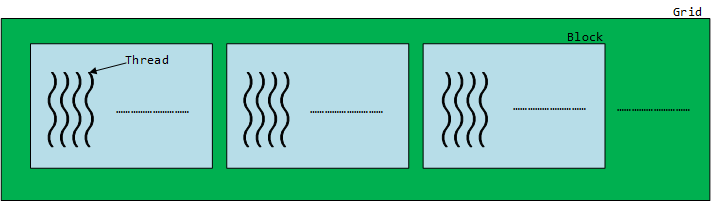
\includegraphics[width=\textwidth]{grid}

The dimensions of the grid and blocks are stated when the kernel is launched. The dimensions are called the \gls{execution configuration}. The example's execution configuration syntax was \verb|<<<2, 512>>>|. The first number is the number of blocks in the grid, which is the grid size. The second number is the number of threads per block, which is the block size. The product of the two gives the total number of threads in the grid. From a programming perspective, \verb|<<<1, 1024>>>| would give the same result. 1024 is also the typical limit of threads per block, but that depends on the compute capability of the device.

Within the kernel code, there are three API variables: threadIdx.x, blockIdx.x, and blockDim.x.\footnote{It is possible to have a 2D or 3D grid where threadIdx.y, threadIdx.z, and the like are used, but this paper will not use them}Using these variables, it's possible to find a unique ID for each thread. 

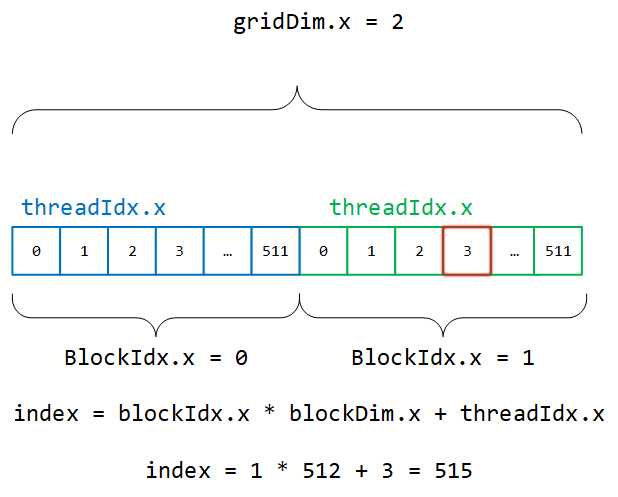
\includegraphics[width=0.95\textwidth]{img/cuda_indexing} 

This unique ID is typically used for indexing, as in my example.
\subsubsection{Hardware Perspective}
\indent From the hardware perspective, each GPU is a collection of memory and compute cores. There are CUDA cores which do arithmetic computations, also known as \glspl{sp}. There are also some special cores dedicated to specific purposes such as double precision operations, transcendental functions, the new Tensor cores for matrix multiplication, and the new raytracing cores. A collection of \glspl{sp} and these special cores make a \gls{sm}. Each \gls{sm}, alongside the cores, have shared memory, warp schedulders, L1 cache, and registers. On some devices, shared memory is physically the same as L1 cache. The entire GPU shares L2 cache, constant memory, and global memory.

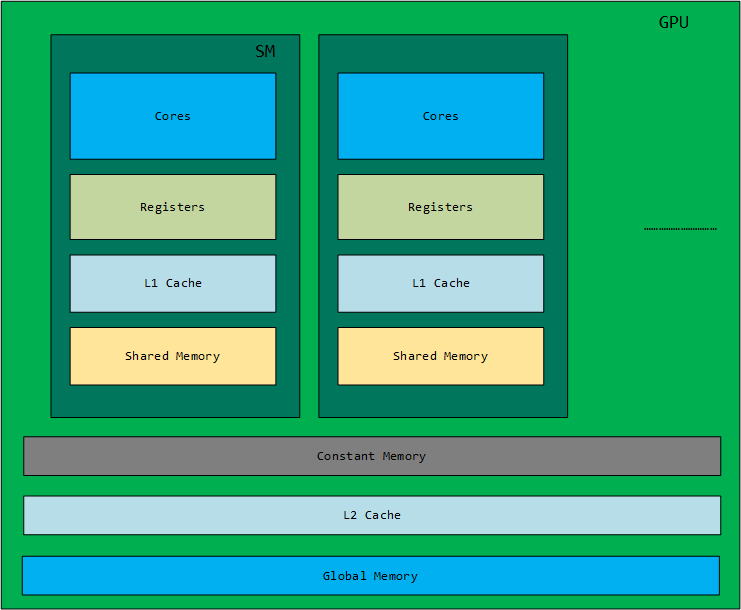
\includegraphics[width=0.95\textwidth]{hardware}

In order of fastest and smallest to slowest and largest, the memory hierarchy goes registers, shared memory, constant memory, and global memory.  This means that access to registers and shared memory is orders of magnitude faster than accessing global memory in terms of number of cycles. There are typically 64 K registers per \gls{sm}, 48 KB of shared memory, 64 KB of constant memory, and anywhere from 2-32GB of memory in global memory. These all depend on the device and the compute capability of the device.

\subsubsection{Where Hardware and Software Meet}
\indent Hardware and software interact through warps. A warp is a group of 32 threads. These 32 threads run in lock step, so each instruction in the 32 threads execute together. If there are less than 32 threads to execute, the warp will still run as if there were 32. Because of this, the number of threads per block should be a multiple of 32. If it's any less, then only a fraction of the warp is being utilized, and performance will take a massive hit. Each \gls{sm} has a specific number of warp schedulers depending on the compute capability of the device. Typically, this is four. \say{Then, at every instruction issue time each scheduler issues one instruction for one of its assigned warps, if any} \citep{cudaC}.

In an example, let's say that a \gls{sm} has 1024 threads running at the same time, which is typically the maximum number of threads per block. Each individual thread is not independent. 32 of them (a warp) are executed in lock step, with each assembly instruction being executed on the warp as a whole. This means that there are 32 warps. If the warps are distributed evenly across the four schedulers, each scheduler is assigned 8 warps. Each scheduler will execute a single lock instruction on one of these 8 warps on every single instruction cycle. Instruction cycles are typically every four clock cycles.The chosen warp becomes known as an active warp. The active warp is chosen purely based off available resources. If an instruction is waiting for memory to arrive from the global memory for 100 cycles, the warp scheduler will not call the next instruction on that particular warp until after those 100 cycles. An example order for the scheduler would be to execute instruction 10 on warp 0, then instruction 7 on warp 3, then instruction 2 on warp 6, then instruction 11 on warp 0. This continues for every instruction cycle as long as there are available resources for the warp, otherwise the scheduler has to wait. 

The amount of time that the schedulers have to wait will depend on the execution configuration(s) of the kernel(s) that are running. Ideally, every scheduler should be running an instruction every single instruction cycle. This is implicitly controlled by how the kernels access memory and how many warps and therefore threads there are per block.
\subsubsection{The Bottlenecks}
There are a several bottlenecks and caveats when programming for GPUs that will impede acceleration. These are the primary issues that I ran into.

\paragraph{Moving Data To/From the GPU} \hspace{0pt} \\
\indent The first issue is getting data on the chip in the first place. The CPU has to tell the memory to move data through the bus and into the \glspl{gpu} main, global memory. This can be done by calling two APIs to allocate memory and transfer memory to the device. Naturally, there is an API to free memory as well \citep{cudaC}.

\begin{minted}[breaklines, breakanywhere]{cuda}
    cudaResult_t cudaMalloc(void** ptr, size_t numberOfBytes);
    cudaResult_t cudaMemcpy(void* dst, void* src, cudaMemcpyKind kind, size_t numberOfBytes);
    cudaResult_t cudaFree(void* ptr);
\end{minted}

The bottleneck is the bus itself, whose transfer protocol is typically \gls{pcie}. GPUs are typically inserted into \gls{pcie} X16 slots on a desktop computer. This means that there are 16 lanes of data that can be transferred in parallel. The speed the different versions of \gls{pcie} are:
\begin{center}
PCIe Bandwidth
\begin{tabular}{ c c c}
Version Number & Bandwidth X1 & Bandwidth X16 \\
1.0 & 250 MB/s & 4 GB/s \\
2.0 & 500 MB/s & 8 GB/s \\
3.0 & 984.6 MB/s & ~15 GB/s \\
4.0 & 1969 MB/s & ~30 GB/s 
\end{tabular}

\citep{pci-sig}
\end{center}
Most motherboards nowadays use \gls{pcie} v3.0. For an example with \gls{pcie} v1.0, in an audio context, 4 GB is approximately an hour and a half of audio in stereo at 96kHz. This means that it will take at least 2 seconds to move the data back and forth - not even to process the data. The later versions of \gls{pcie} have faster bandwidth, but nowhere near close to the speed of the \gls{gpu}. This is why data sets should contain at least one million elements to make it worth \gls{gpu} acceleration. One million is a ballpark number peak where the CPU can computer faster than it takes for the data set to travel to and from the \gls{gpu}. For time domain convolution, my threshold number was 1024 elements. For frequency domain convolution, my threshold number was 8.3 million elements.

\paragraph{Global Memory Access} \hspace{0pt} \\
\indent The second issue comes after the data is on the \gls{gpu} chip. Global memory on the chip is anywhere from 2 GB to 32 GB. That's a worthwhile amount of memory, but the global memory is not directly connected to the cores. Global memory access is also the slowest type of memory access on a \gls{gpu}. This means that if all the threads need global memory access, there's a higher probability of the warp schedulers needing to wait for the memory to come to the cores. For example, a global memory access request may take 128 cycles to process. An instruction cycle is typically 4 cycles. Let's go back to the previous example where a SM has 1024 threads and 4 warp schedulers, so that there are 32 warps with 8 warps per scheduler. Lets say that instruction 1 is calculating the unique global ID: \verb|int threadID = blockIdx.x * blockDim.x + threadIdx.x|, instruction 2 is retrieving memory, and instruction 3 is incrementing the value. Let's also pretend that instruction 1 takes 8 cycles, or 2 instruction cycles. A single scheduler's instruction cycle could look like this:
\newpage
\begin{center}
Example Warp Scheduler Instruction Sequence
\begin{tabular}{ c c c}
 Instruction Cycle Number & Warp Number & Instruction Number\\ 
 1 & 0 & 1 \\  
 2 & 4 & 1 \\
 3 & 0 & 2 (must wait 32 cycles) \\
 4 & 7 & 1 \\
 5 & 2 & 1 \\
 6 & 4 & 2 (must wait 32 cycles) \\
 7 & 1 & 1 \\
 8 & 7 & 2 (must wait 32 cycles) \\
 9 & 3 & 1 \\
 10 & 2 & 2 (must wait 32 cycles) \\
 11 & 5 & 1 \\
 12 & 1 & 2 (must wait 32 cycles) \\
 13 & 3 & 2 (must wait 32 cycles) \\
 14 & 6 & 1 \\
 15 & 5 & 2 (must wait 32 cycles) \\
 16 & 6 & 2 (must wait 32 cycles) \\
 17 & waiting, no ready warps & \\
 18 & waiting, no ready warps & \\
 19 & waiting, no ready warps & \\
 20 & waiting, no ready warps & \\
 ......... & ......... & ......... \\
 35 & 0 & 3 \\
 36 & waiting, no ready warps & \\
 37 & waiting, no ready warps & \\
 38 & 4 & 3 \\
 39 & waiting, no ready warps & \\
 40 & 7 & 3 \\
 41 & waiting, no ready warps & \\
 42 & waiting, no ready warps & \\
 43 & waiting, no ready warps & \\
 44 & 1 & 3 \\
 45 & 3 & 3 \\
 46 & waiting, no ready warps & \\
 47 & 5 & 3 \\
 48 & 6 & 3
\end{tabular}
\end{center}

Half the instruction cycles are just waiting for data. This is far from ideal and is actually a 2x slowdown from the ideal. Because of this, there is a term called \gls{cgma}. This is a ratio of memory accesses to computations in a kernel. In my increment example, the \gls{cgma} was 1. The higher the \gls{cgma}, the better the performance \citep{kirk_hwu_2010}.

\subsubsection{Optimization Techniques}
\paragraph{Streams} \hspace{0pt} \\
\indent Streams are a software concept and \gls{cuda} \gls{api} for a queue of commands. In \gls{cuda}, streams are used to manage execution order and overlap of kernels and memory copies. By using streams, different tasks on the \gls{gpu} that would typically run sequentially can run in parallel. Streams can be created, synchronized, and destroyed throughout the program through these APIs \citep{cudaC}:
\begin{minted}[breaklines, breakanywhere]{cuda}
    cudaResult_t cudaStreamCreate(cudaStream_t* stream);
    cudaResult_t cudaStreamQuery(cudaStream_t stream);
    cudaResult_t cudaStreamSynchronize(cudaStream_t stream);
    cudaResult_t cudaStreamDestroy(cudaStream_t stream);
\end{minted}
The two most frequent applications of streams are for asynchronous memory copies and concurrent kernels. 
\subparagraph{Asynchronous Memory Copy} \hspace{0pt} \\
\indent Memory needs to be transferred from the host to the device, and this is one of the primary bottlenecks of \gls{gpu} computing, as detailed in the previous section. The API to transfer memory to the device is \citep{cudaC}:

\begin{minted}[breaklines, breakanywhere]{cuda}
    cudaResult_t cudaMemcpy(void** dst, void* src, cudaMemcpyKind kind,size_t numberOfBytes);
\end{minted}

This is an example of a synchronous API call, compared with an asynchronous API call. Synchronous means that it will prevent the program from progressing any further until this call has finished. Asynchronous means that control will return back to the host immediately after launch, allowing this task to finish in the meanwhile. There is an asynchronous flavor of \verb|cudaMemcpy()| \citep{cudaC}:

\begin{minted}[breaklines, breakanywhere]{cuda}
cudaResult_t cudaMemcpyAsync(void** dst, void* src, cudaMemcpyKind kind, size_t numberOfBytes, cudaStream_t stream);
\end{minted}
    
The caveat with asynchronous memory transfers is that it requires pinned memory. Pinned memory is an allocated section of RAM that can't be paged out to the disk. Pages are a virtual memory concept. Essentially, some processes have sections of memory that are stored on the disk to allow multiple processes to run independently, thinking that each has all of the physical memory available. Paging also allows the less frequently used memory to be stored in a location with larger capacity. The problem with pinned memory is that allocating too much of it will slow the process and all other processes running at the same time. Pinned memory is allocated and freed through CUDA APIs \citep{cudaC}:

\begin{minted}[breaklines, breakanywhere]{cuda}
    cudaResult_t cudaMallocHost(void** ptr, size_t numberOfBytes);
    cudaResult_t cudaFreeHost(void* ptr);
\end{minted}

My program combines synchronous and asynchronous memory transfers when moving the data to the device. Here is an abridged version of the code:

\begin{minted}[breaklines, breakanywhere]{cuda}
    cudaStream_t streams[4];
    float *d_ibuf, *ibuf;
    
    /*Open input file for reading*/
    SF_INFO i_info;
    SNDFILE *i_sndfile;
    i_sndfile = sf_open("input.wav", SFM_READ, &i_info);
	
	
    /*long long * iframes is defined as the size of the input
      long long * new_size is defined as pow(2, ceil(log2(N + K - 1)))
      checkCudaErrors(cudaResult_t) is an exception handler that will stop
        the program and print the error if an error occurs*/
    int mod = *iframes % 2;
    
    ...
    
    /*Allocate pinned memory*/
    checkCudaErrors(cudaMallocHost((void**)&ibuf, (*iframes / 2 + mod) * sizeof(float)));

    /*Allocate device memory*/
    checkCudaErrors(cudaMalloc(d_ibuf, *new_size * sizeof(float)));
    
    /*Create streams*/
    for(int i = 0; i < 4; i++){
        checkCudaErrors(cudaStreamCreate(&streams[i]));
	}
    
    ...
    
	/*Read in half of input*/
	sf_read_float(i_sndfile, ibuf, totalSize / 2);
	checkCudaErrors(cudaMemcpyAsync(*d_ibuf, ibuf, totalSize / 2 * sizeof(float), cudaMemcpyHostToDevice, streams[3]));

	...
	if(cudaStreamQuery(streams[3]) == cudaSuccess){
	    /*Read in other half of input*/
	    sf_read_float(i_sndfile, ibuf, totalSize / 2 + mod);
	    checkCudaErrors(cudaMemcpyAsync(*d_ibuf + totalSize / 2, ibuf, (totalSize / 2 + mod) * sizeof(float), cudaMemcpyHostToDevice, streams[3]));
	    ...
	    /*Do other things on the host*/
        ...
	}
	else{
	    ...
	    /*Do other things on the host*/
	    ...
	    /*Read in other half of input*/
	    sf_read_float(i_sndfile, ibuf, totalSize / 2 + mod);
	    checkCudaErrors(cudaMemcpyAsync(*d_ibuf + totalSize / 2, ibuf, (totalSize / 2 + mod) * sizeof(float), cudaMemcpyHostToDevice, streams[3]));
	}
	
\end{minted}

My code compromises between fully asynchronous memory transfers and a smaller pinned memory. I am expecting my input to grow very large, up to $2^{30}$ samples or $2^{32}$ bytes for my experiment, so I chose to only allocate half the amount of pinned memory required. Because of that, the first \verb|cudaMemcpy()| has to be synchronized before the second half of the audio can be read. Otherwise, the second call to \verb|sf_read_float| would overwrite the data while it's being transferred.

\subparagraph{Concurrent Kernels} \hspace{0pt} \\
\indent Another use for streams are for concurrent kernels. Kernel launches are asynchronous, but several kernel launches will proceed sequentially on the device. They do not run at the same time if called immediately after each other. Instead, the two kernels will be in a queue. Sometimes this is desired - for instance if two kernels affect the same data - and other times it is not, especially if the device is large enough to fit multiple grids. 

The number of concurrent kernels that can run on the device depends heavily on the compute capability, but it is typically 32. Other devices allow for 4, 16, and 128. Streams need to be created and added to the \gls{execution configuration} in order to allow concurrent kernels. 

\subparagraph{Full Example Of Streams} \hspace{0pt} \\
\begin{minted}[breaklines, breakanywhere]{cuda}
    /*input parameters that will get returned to the caller include 
      long long *iframes, long long *fframes, 
      float **d_ibuf, float **d_fbuf, 
      long long *new_size 
      
      input parameters given to this function include 
      const char *iname, const char *fname
      */
      
	cudaStream_t streams[4];
	float *ibuf, *fbuf;
	SF_INFO i_info, f_info;
	SNDFILE *i_sndfile, *f_sndfile;
	

	/*Read input*/
	i_sndfile = sf_open(iname, SFM_READ, &i_info);

	/*Read reverb*/
	f_sndfile = sf_open(fname, SFM_READ, &f_info);
	
	/*Store number of frames*/
	*iframes = i_info.frames;
	*fframes = f_info.frames;
	
	int mod = *iframes % 2;
	
	/*Find padded size for FFT*/
	*new_size = pow(2, ceil(log2((double)(*iframes + *fframes - 1))));
	
	/*Allocate device memory*/
	checkCudaErrors(cudaMalloc(d_ibuf, *new_size * sizeof(float)));
	checkCudaErrors(cudaMalloc(d_fbuf, *new_size * sizeof(float)));
	
	/*Allocate host pinned memory for input and filter*/
	checkCudaErrors(cudaMallocHost((void**)&ibuf, *iframes / 2 + mod * sizeof(float)));
	checkCudaErrors(cudaMallocHost((void**)&fbuf, *fframes * sizeof(float)));
	
	/*Create streams*/
	for(int i = 0; i < 4; i++){
		checkCudaErrors(cudaStreamCreate(&streams[i]));
	}
	
	/*Pad buffers with zeros*/
	/*FillWithZeros is a kernel that takes in a pointer, start element, and end element. All values from start to end become 0*/
	int numThreads = 512;
	int numBlocks = (*new_size - *fframes  + numThreads - 1) / numThreads;
	FillWithZeros<<<numBlocks, numThreads, 0, streams[0]>>>(*d_fbuf, *fframes,  *new_size);
	
	numBlocks = (*new_size - *iframes + numThreads - 1) / numThreads;
	FillWithZeros<<<numBlocks, numThreads, 0, streams[1]>>>(*d_ibuf, *iframes, *new_size);
	
	/*Read in half of input*/
	sf_read_float(i_sndfile, ibuf, totalSize / 2);
	checkCudaErrors(cudaMemcpyAsync(*d_ibuf, ibuf, totalSize / 2 * sizeof(float), cudaMemcpyHostToDevice, streams[3]));

	/*Read in all filter audio data*/
	sf_read_float(f_sndfile, fbuf, *fframes);

	/*Fill filter buffer*/
	checkCudaErrors(cudaMemcpyAsync(*d_fbuf, fbuf, *fframes * sizeof(float), cudaMemcpyHostToDevice, streams[2]));
	
	if(cudaStreamQuery(streams[3]) == cudaSuccess){
		/*Read in other half of input*/
		sf_read_float(i_sndfile, ibuf, totalSize / 2 + mod);
		checkCudaErrors(cudaMemcpyAsync(*d_ibuf + totalSize / 2, ibuf, (totalSize / 2 + mod) * sizeof(float), cudaMemcpyHostToDevice, streams[3]));
		checkCudaErrors(cudaStreamSynchronize(streams[2]));
		checkCudaErrors(cudaStreamDestroy(streams[2]));
		checkCudaErrors(cudaFreeHost(fbuf));
		sf_close(f_sndfile);
	}
	else{
		checkCudaErrors(cudaStreamSynchronize(streams[2]));
		checkCudaErrors(cudaStreamDestroy(streams[2]));
		checkCudaErrors(cudaFreeHost(fbuf));
		sf_close(f_sndfile);

		/*Read in other half of input*/
		checkCudaErrors(cudaStreamSynchronize(streams[3]));
		sf_read_float(i_sndfile, ibuf, totalSize / 2 + mod);
		checkCudaErrors(cudaMemcpyAsync(*d_ibuf + totalSize / 2, ibuf, (totalSize / 2 + mod) * sizeof(float), cudaMemcpyHostToDevice, streams[3]));		
	}
	/*Synchronize and destroy the rest of the streams*/
	for(int i = 0; i < 4; i++){
		if(i == 2) continue;
		checkCudaErrors(cudaStreamSynchronize(streams[i]));
		checkCudaErrors(cudaStreamDestroy(streams[i]));
	}	
	sf_close(i_sndfile);
	checkCudaErrors(cudaFreeHost(ibuf));
\end{minted}

Here, I have 4 streams, because there is a potential for 4 items to run concurrently: padding the filter with 0's, padding the input with 0's, copying the filter to the device, and copying the input to the device. Using streams, the program can hide the bottleneck of moving data to the \gls{gpu} by running \gls{cpu} functions at the same time.
\paragraph{Shared Memory} \hspace{0pt} \\
\indent In the past examples with streams and concurrent kernels, the third parameter of the execution configuration has been 0. That third parameter is actually to specify the amount of shared memory per block for each kernel. Shared memory, as discussed in the hardware perspective of \glspl{gpu}, is memory that is on each \gls{sm}. Because of this, accessing shared memory is significantly faster than accessing global memory. Shared memory can be declared statically inside the kernel such as \verb|__shared__ float x[512]| or dynamically in the third parameter of the execution configuration. Once declared, each thread in the block can load data into that shared memory at the same time and then use it. 

\begin{minted}[breaklines, breakanywhere]{cuda}
#define TILE 512
__global__ kernel(float *d_buf, int N){
    __shared__ data[TILE];
    int threadID = blockIdx.x * blockDim.x + threadIdx.x;
    
    if(threadID < N){
        data[threadIdx.x] = d_buf[threadID];
    }
    __syncthreads();
    
    /*Do some calculation with tile and store back in d_buf*/
}

... 
    /*N = size of d_buf*/
    int B = (N + TILE - 1) / TILE;
    kernel<<<B, TILE>>>(d_buf, N);
...
\end{minted}

\verb|__syncthreads()| is an API that will synchronize all of the threads in a block before proceeding. This barrier is there to make sure that \verb|data[]| is loaded with information before doing any calculations. I attempted to use shared memory for time domain convolution. However, this algorithm turned out to be less effective after timing tests.

\begin{minted}[breaklines, breakanywhere]{cuda}
#define tile 512
__global__ void timeDomainConvolutionExcessive(float *ibuf, float *fbuf, float *obuf, long long iFrames, int chunkNo){
	__shared__ float x[tile];
	__shared__ float h;
	
	if(chunkNo * tile + threadIdx.x < iFrames){
		x[threadIdx.x] = ibuf[chunkNo * tile + threadIdx.x];
	}
	h = fbuf[blockIdx.x];
		__syncthreads();
	if(chunkNo * tile + threadIdx.x < iFrames){
		atomicAdd(obuf + blockIdx.x + chunkNo * tile + threadIdx.x, x[threadIdx.x] * h);
	}
}
...
    /*main/caller*/
    int numChunks = (iFrames + tile - 1) / tile;
    cudaStream_t streams[numChunks];
    for(int i = 0; i < numChunks; i++){
        checkCudaErrors(cudaStreamCreate(&streams[i]));
        timeDomainConvolutionExcessive<<<fFrames, tile, 0, streams[i]>>>(d_ibuf, d_fbuf, d_obuf, iFrames, i);
    }
\end{minted}

\verb|atomicAdd()| takes in the address of what to add and the value to add that by. \verb|atomicAdd| prevents race conditions among different blocks by fusing the read, add, and write operations into a single instruction.

This algorithm is based off the cache-friendly time domain algorithm:
\begin{minted}[breaklines, breakanywhere]{cuda}
for k [0, K):
    for n [0, N):
        y[k + n] += x[n] * h[k]
\end{minted}
It divided the input into chunks of length \verb|tile|. There are \verb|fFrames| number of blocks, and each block corresponded to a point in the filter. 

This was an attempt to use shared memory, but it was ultimately not used because it was less accurate and slower. 
\paragraph{Memory Coalescing} \hspace{0pt} \\
\indent Memory coalescing builds off the concept of writing cache-friendly code, as discussed in the Sequential Time Domain Convolution section. Memory coalescing happens when the threads in a warp require sequential global memory access, such as threads 0 - 31 accessing elements 0 - 31 in an array of floats, respectively. The memory needs to be brought up from the global memory to L1 cache inside the \gls{sm}, and cache comes in blocks. An entire block of 128 bytes (32 elements if they are floats/ints) will be brought up from global memory to L1 cache. The best case scenario is that elements 0 - 31 land perfectly in this cache block. In that case, 32 global memory requests from a warp were \textit{coalesced} into a single global memory transaction. 

To try to coalesce global memory accesses, data should always be accessed sequentially among the threads. This will only happen with primitive data types like ints or floats. Structures might not land perfectly in the block since they contain primitive data types. This is known as alignment. The best case scenario is if access is aligned and also sequential. Otherwise, it will take at least two cache blocks to bring the 32 items. Memory allocated through \verb|cudaMalloc()| are guaranteed to be aligned to 256 bytes, so element 0, 32, 64, 96, etc of any array of floats is guaranteed to fall in the beginning of a cache block \citep{cudaCBestPractices}.

Memory coalescing is a tool and technique to help with the bottleneck of global memory access. It does complicate indexing within kernels. For instance, my kernel from above contained the line
\begin{minted}[breaklines, breakanywhere]{cuda}
atomicAdd(obuf + blockIdx.x + chunkNo * tile + threadIdx.x, x[threadIdx.x] * h);
\end{minted}

\verb|obuf + blockIdx.x + chunkNo * tile + threadIdx.x| is the entire line to calculate the position in the output that this thread is going to calculate. A visual cue to see if memory will be coalesced is to make sure that there is a \verb|+ threadIdx.x| and that \verb|threadIdx.x| is not multiplied by anything. That way, when threadIdx.x increments by one, the output pointer also increments by one. 

\paragraph{Scatter vs. Gather Decomposition} \hspace{0pt} \\
\indent For problems where the output requires multiple values of the input, such as time domain convolution, there are two ways to approach the problem. The first is a \say{gather-oriented approach} and the second is a \say{scatter-oriented approach} \citep{6216339}. The cache-unfriendly time domain convolution code is an example of a gather-oriented approach when the algorithm is parallelized:
\begin{minted}{cpp}
Gather Decomposition (Sequential)

for n [0, Y):
    value = 0
    for k [0, K):
        if (n - k < x.length):
            value += x[n - k] * h[k]
    n = value

\end{minted}
\begin{minted}[breaklines, breakanywhere]{cuda}
Gather Decomposition (Parallel)
__global__ void timeDomainConvolution(float *ibuf, float *fbuf, float *obuf, long long iFrames, long long fFrames){
    int threadID = blockIdx.x * blockDim.x + threadIdx.x;
    if(threadID < iFrames + fFrames - 1){
        float value = 0.0f;
        for(int k = 0; k < fFrames; k++){
            if (threadID - k > = 0 && threadID - k < iFrames){
                value += ibuf[threadID - k] * fbuf[k];
            }
        }
        obuf[threadID] = value;
    }
}
...
Eeach thread indexes an output element
\end{minted}
The cache-friendly algorithm for time domain convolution is considered a scatter decomposition.

\begin{minted}{cpp}
Scatter Decomposition (Sequential)
for k [0, K):
    for n [0, N):
        y[k + n] += x[n] * h[k]
\end{minted}
\begin{minted}[breaklines, breakanywhere]{cuda}
Scatter Decomposition (Parallel)
__global__ void timeDomainConvolutionAtomic(float *ibuf, float *fbuf, float *obuf, long long iFrames, long long fFrames){
    int threadID = blockIdx.x * blockDim.x + threadIdx.x;
	float h;
	if(threadID < fFrames){
		h = fbuf[threadID];
		for(int i = 0; i < iFrames; i++){
			atomicAdd(obuf + threadID  + i , ibuf[i] * h);
		}
	}
...
Each thread indexes a filter element
\end{minted}

Gather decompositions are better when parallelized because each thread writes to an independent output address. Scatter decompositions often suffer performance issues, because several threads write to the same output addresses. When multiple threads are writing to the same output address, there's a possibility of race conditions which will give unexpected answers. For instance, if two threads try to increment an address at the same exact time, the threads could write to their respective caches the new value. Then the value gets copied into main memory twice - resulting in only a single increment instead of two increments. \verb|atomicAdd()| ensures that the read, add, and write operations happen in one instruction so that another threads' read, add, and write operations will not interleave with the previous one. The problem with \verb|atomicAdd()| is that it will sequentialize parallel code. If several threads want to increment an address, \verb|atomicAdd()| forces them to queue, which will take a performance hit. 

For these two examples of algorithms, the gather decomposition is better even though memory is not necessarily being coalesced (in \verb|ibuf[threadID - k]|. \verb|fbuf[k]| is coalesced).